\subsection{Equation selection and shared reductions at higher loop orders}
\label{sec:higher-loop-acceleration}
The preceding native comparisons cover specific structures with two or three loops. To study the higher orders already present in the integral
collection, we now use the coupled vacuum family in
Eq.~\eqref{eq:coupled-vacuum}. This family has one power of each massless
denominator and two to four distinct massive denominators that depend on
the same momentum \(Q\). Its Euler identities and mass partial fractions
remain valid for any positive integer number of loops. This structure
allows us to test every order from one through twelve with an exact
reference, while keeping the family restriction explicit.

The dependence on the loop order suggests a further reduction in repeated
work. Let \(B=\sum_j b_j\), retain the squared-mass scale \(\mu\), and define
\begin{equation}
 z=L(d-2),\qquad
 W^{(L)}_{\boldsymbol b}=\mu^{B-1}V^{(L)}_{\boldsymbol b}.
 \label{eq:loop-shared-variable}
\end{equation}
The rescaling gives every \(W^{(L)}_{\boldsymbol b}\) the same mass dimension
as the masters \(M_j^{(L)}\). Equations~\eqref{eq:higher-loop-euler} and
\eqref{eq:higher-loop-partial-fraction} then become
\begin{align}
 0&=(z-2B)W^{(L)}_{\boldsymbol b}
       +2\sum_j b_j\rho_j W^{(L)}_{\boldsymbol b+\boldsymbol e_j},
 \label{eq:loop-shared-euler}\\
 0&=(\rho_i-\rho_j)W^{(L)}_{\boldsymbol b}
       -W^{(L)}_{\boldsymbol b-\boldsymbol e_i}
       +W^{(L)}_{\boldsymbol b-\boldsymbol e_j}.
 \label{eq:loop-shared-mass}
\end{align}
Here \(\rho_j\) is the positive squared-mass ratio defined earlier, and the
second identity requires \(b_i,b_j>0\).
The coefficient equations depend on \(L\) only through \(z\). We can
therefore solve one system over \(\mathbb Q(z)\) at fixed rational mass
ratios and obtain
\begin{equation}
 V^{(L)}_{\boldsymbol b}
 =\mu^{1-B}\sum_{j=1}^{R}
 C_{\boldsymbol b j}\bigl(L(d-2);\boldsymbol\rho\bigr)M_j^{(L)}.
 \label{eq:loop-shared-result}
\end{equation}
Each \(C_{\boldsymbol b j}\) is a polynomial in \(z\) with rational
coefficients in the present domain. The master integrals retain their
physical dependence on \(L\). The shared calculation supplies their
reduction coefficients.

We next reduce the number of identities passed to Kira. For a mixed
integral, the model scores each allowed pair \((i,j)\) in
Eq.~\eqref{eq:loop-shared-mass}. The selected identity replaces that integral
with two integrals of total massive power \(B-1\). We repeat the choice for
the resulting integrals and merge repeated dependencies across the target
batch. An integral with only one massive denominator uses
Eq.~\eqref{eq:loop-shared-euler} at the seed
\((k-1)\boldsymbol e_j\) to reduce power \(k\). At \(B=1\), the integral
belongs to the prescribed master basis. This decreasing total power
proves termination and sufficiency for every allowed model choice. Mass
partial fractions carry no IBP seed; the saved dependency choices also
determine the actual Euler seeds with one massive denominator.

The training reference counts the distinct nonmaster integrals in
recursively chosen dependency sets. If \(\mathcal D(\boldsymbol b)\)
denotes such a set, the candidate cost is
\begin{equation}
 c(\boldsymbol b;i,j)=
 \left|\{\boldsymbol b\}\cup
 \mathcal D(\boldsymbol b-\boldsymbol e_i)\cup
 \mathcal D(\boldsymbol b-\boldsymbol e_j)\right|.
 \label{eq:loop-choice-teacher}
\end{equation}
Every pair tied for the smallest candidate cost receives label one.
The recursion fixes a valid local reference and does not establish the
minimum cost for an entire target batch. We train small classification
trees using the ordered massive powers, pair positions, active-denominator
count and simple power summaries. There are 18 features, with no loop order
feature. The absence of \(L\) follows from
Eqs.~\eqref{eq:loop-shared-euler}--\eqref{eq:loop-shared-mass}.
A leaf score is an empirical training frequency. The runtime selects the
highest score and uses exact identities for the algebra. For two active
massive denominators, the single available pair is selected directly.

The training set contains 2,016 candidate actions in
546 exponent shapes, with total power through nine.
We fit depth limits four, eight and twelve using a minimum child size of
four examples. Validation selects the depth-4 candidate, which
contains 15 nodes. On 277 distinct development coefficients, the reader
agrees with symbolic algebra and takes 0.159 seconds,
compared with 4.149 seconds for the symbolic
reader. This reading improvement applies to every comparison arm and is
separate from the learned decision.


Kira solves each selected system through its interface for supplied
systems~\cite{Kira2,Kira3}. We generate the Euler and mass identities
within the measured workflow and use the same native elimination policy
for every comparison arm. This experiment measures supplied-identity
reductions. It does not measure Kira's native generation of a general
IBP system at higher loop orders. The earlier native benchmarks retain that separate
role.

The integration reads the exported coefficients with bounded rational
polynomial arithmetic and checks that polynomial division leaves zero
remainder. Development comparisons against symbolic algebra check this
reader independently. The final check uses the Taylor partial fraction
formula in Eq.~\eqref{eq:higher-loop-reference}, which does not follow the
selected dependency path. The workflow rejects unresolved nonmaster
integrals and retains a fallback to the full equation pool. Timings include input and
model loading, selection, equation construction, Kira, coefficient reading,
substitution, verification and any fallback. We also report external
process times, which include Python startup and evidence writing.
Queue waiting time and offline training are excluded.

The refined validation contains 144 workflows on six batches of mass profiles.
It compares the three trees with first-pair, smallest-pair, largest-pair and
extreme-pair rules and the full pool. Each candidate has three repetitions.
The extreme-pair rule chooses an active denominator with the smallest
power and one with the largest power. Validation selects the
extreme route; the selected learned candidate costs
1.7\% more than the selected rule.
We freeze sources, weights, profiles and target lists before 90 reserved
workflows. The reserved set has two profiles for each of
\(R=2,3,4\), with maximum powers eight and twelve, and runs every
\(L=1,\ldots,12\). Some exponent shapes with lower powers also occur in
training; the cases with maximum power twelve extend its power bound. The tests vary
mass profiles within the same topology and do not test new graph classes.
We use three repetitions and report geometric means of the six ratios of
batch medians. Descriptive intervals resample those six batches.


For each mass profile and target batch, we compare separate reductions with the full equation pool at each \(L\), separate learned reductions, a shared reduction with the full equation pool in \(z\), a shared reduction with a simple rule, and a shared learned
reduction. The full pool contains Euler seeds through the largest target
power and all mass-pair identities through one additional power. The
control with a simple rule uses the rule selected on validation. All arms use the
same project Kira binary with the earlier runtime improvements and native
row choices. These controls separate the benefit of exact loop reuse from
the benefit of selecting a smaller equation set.

For separate reductions at each loop order, learned selection gives
a complete-time ratio of 0.911 to the full pool, with
descriptive interval \([0.815,0.986]\).
With exact loop reuse in both arms, learned selection gives a ratio of
0.925 to the shared full pool, with interval
\([0.889,0.958]\).
The learned/shared ratio to the rule/shared control is
0.968, with interval
\([0.927,1.003]\).
These comparisons keep the incremental learned effect separate from
the exact reuse of coefficient equations.

The deployed shared route gives a complete-time ratio of
0.155 to separate reductions with the full equation pool, with interval
\([0.132,0.184]\).
This corresponds to 6.47 times faster execution of the
twelve-order workload under the stated timing definition.
Figures~\ref{fig:higher-loop-complete-time} and
\ref{fig:higher-loop-equations} show the batch costs and equation counts.
Validation fixes the deployed rule before these tests; we retain the
learned results as a measured alternative.

We separate calculation time from the cost of starting Python and archiving
the test evidence. Before those two outer costs, the separate learned
route has time ratio 0.943, with descriptive interval
\([0.873,0.995]\), to the full pool.
The time spent inside Kira has ratio 0.965, with interval
\([0.925,0.992]\).
Thus the calculation saves 5.7\% and Kira itself saves
3.5\% in this comparison. Archiving fewer source
equations contributes to the larger saving in external process time.

With shared coefficients, the ratio of calculation times of the learned route
to the full pool is 0.966, with interval
\([0.941,0.982]\).
Its ratio to the control with a simple rule is 0.997, with interval
\([0.984,1.011]\).
This comparison does not establish an added advantage over the simple rule.
The deployed shared calculation has ratio 0.128 to separate
calculations with the full equation pool, with interval
\([0.102,0.164]\).
The exact change of variable supplies the main reduction in repeated work.


\begin{figure}[htbp]
 \centering
 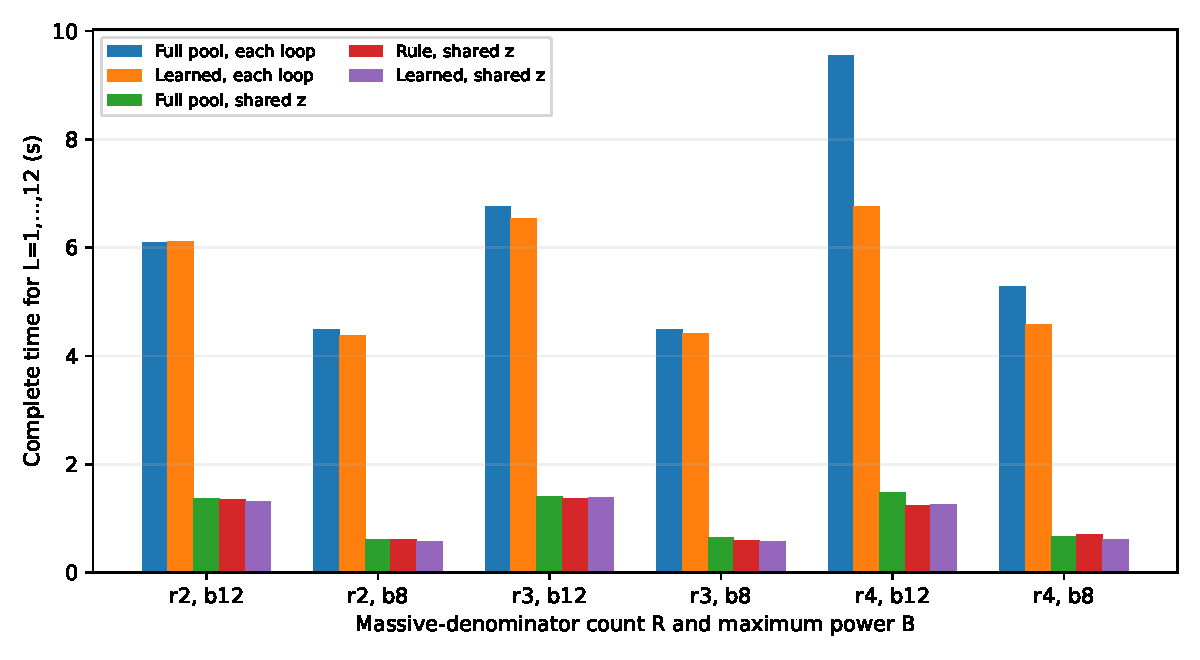
\includegraphics[width=0.98\textwidth]{figures/higher_loop_complete_times.pdf}
 \caption{Median external complete times for the twelve loop orders in
 each reserved batch. Each bar includes the full cost of its stated
 workflow. The shared methods solve once in \(z\) and check the substituted
 coefficients separately at every requested loop order.}
 \label{fig:higher-loop-complete-time}
\end{figure}

\begin{figure}[htbp]
 \centering
 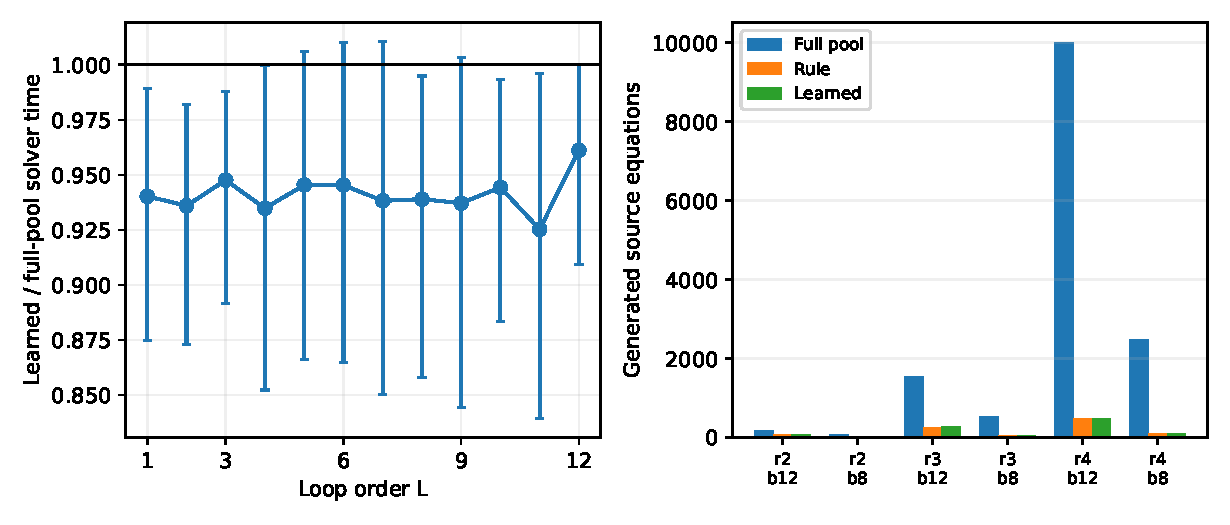
\includegraphics[width=0.98\textwidth]{figures/higher_loop_equations.pdf}
 \caption{Separate-loop solver-time ratios and generated equation counts.
 The left panel includes construction, prediction, Kira and coefficient
 reading for each loop order; the complete workflow also includes the
 checks shown in Fig.~\ref{fig:higher-loop-complete-time}. The intervals
 describe variation across the six reserved batches.}
 \label{fig:higher-loop-equations}
\end{figure}

All 90 reserved workflows and six additional applications pass exact
checks. The extra applications use loop orders 13, 16, 24 and 32.
The audit checks 65,504 coefficient positions, including
5,696 distinct positions, across
492 Kira calls. It finds 0 failed attempts
and 0 fallback workflows.
The largest sampled memory of Kira and its child processes is
23.05 MiB, and the largest temporary
solver storage is 0.58 MiB.
The analytic reference also supplies a direct reduction for this
special family. The reported comparisons measure routes that use Kira.


Equation~\eqref{eq:loop-shared-result} holds for any positive \(L\) in this
scalar family. The finite tests cover the stated orders. Generic scattering
families contain additional scalar products, numerator powers and kinematic
variables, so their native IBP reduction needs separate tests. These results
apply to the stated coupled vacuum family and supplied
identities~\cite{KiraHigherLoopData}.
